\section{Ergebnisse}

\subsection{Vorhersage der Daten\"ubertragungsraten}

\subsubsection{Extreme Gradient Boosting}

\begin{figure}
\centering
\begin{subfigure}{\textwidth}
    \centering
    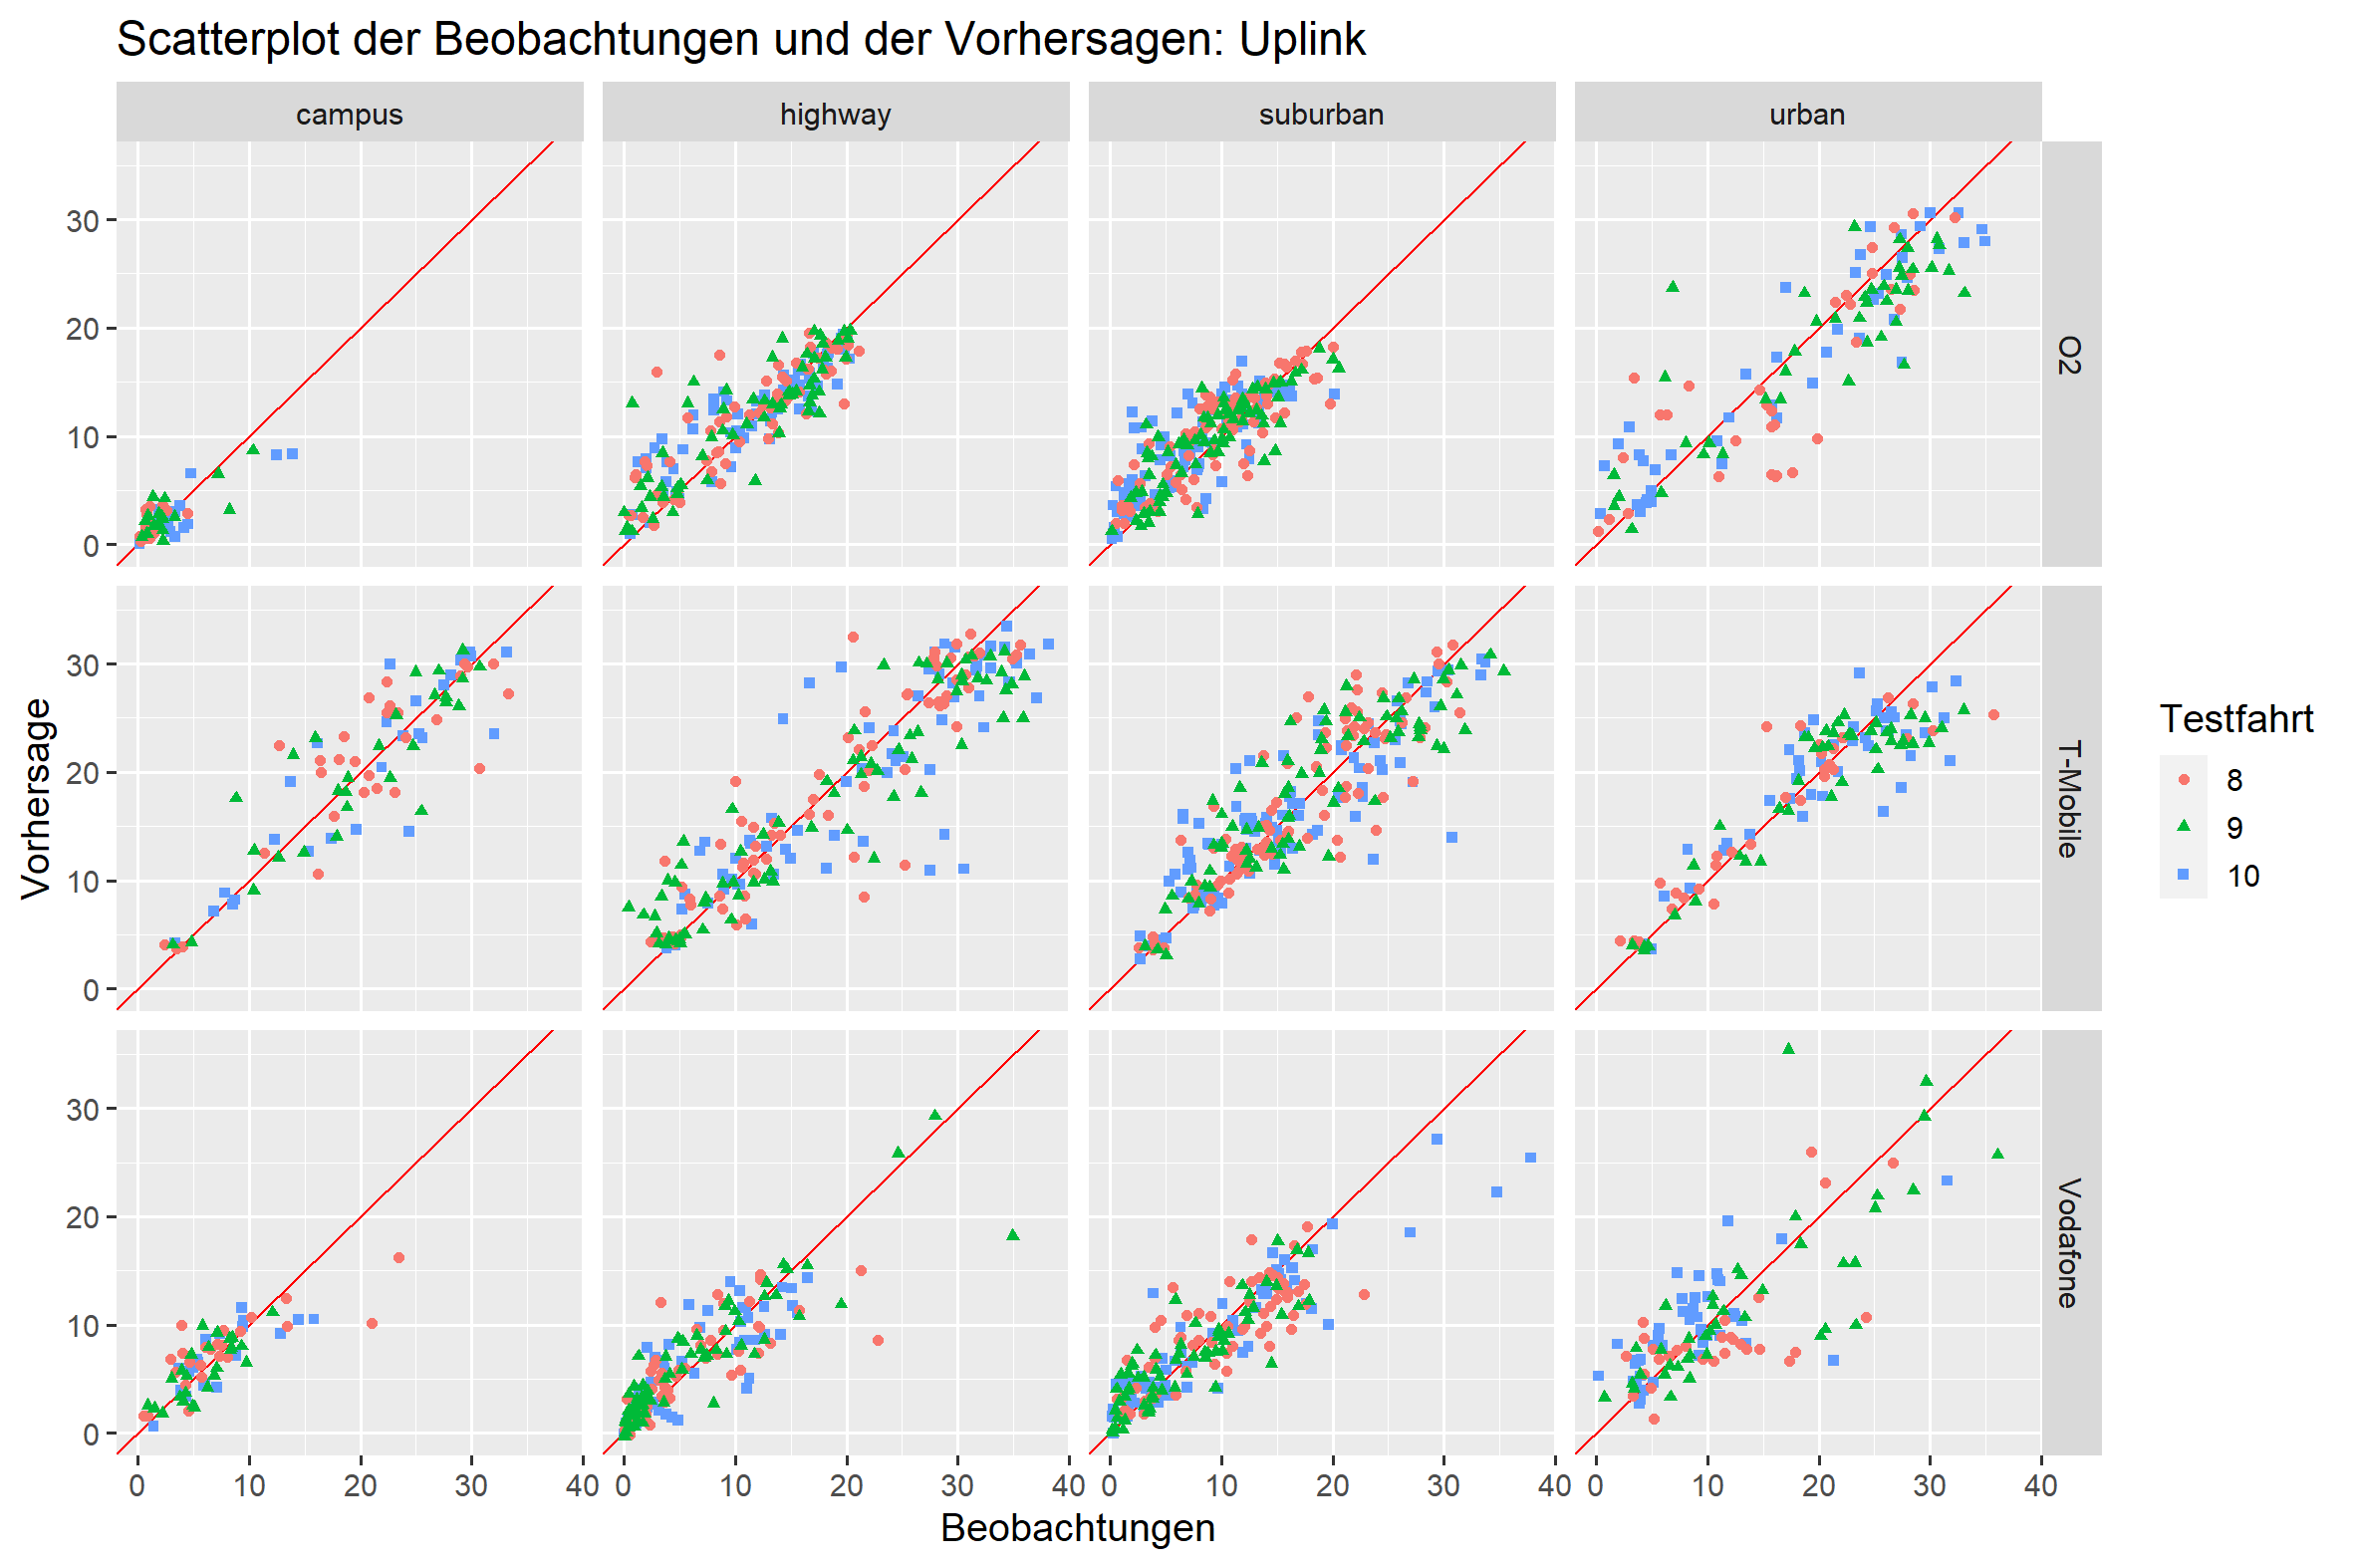
\includegraphics[width=\textwidth]{abbildungen/xgboost_predictions_ul}
\end{subfigure}
\begin{subfigure}{\textwidth}
    \centering
    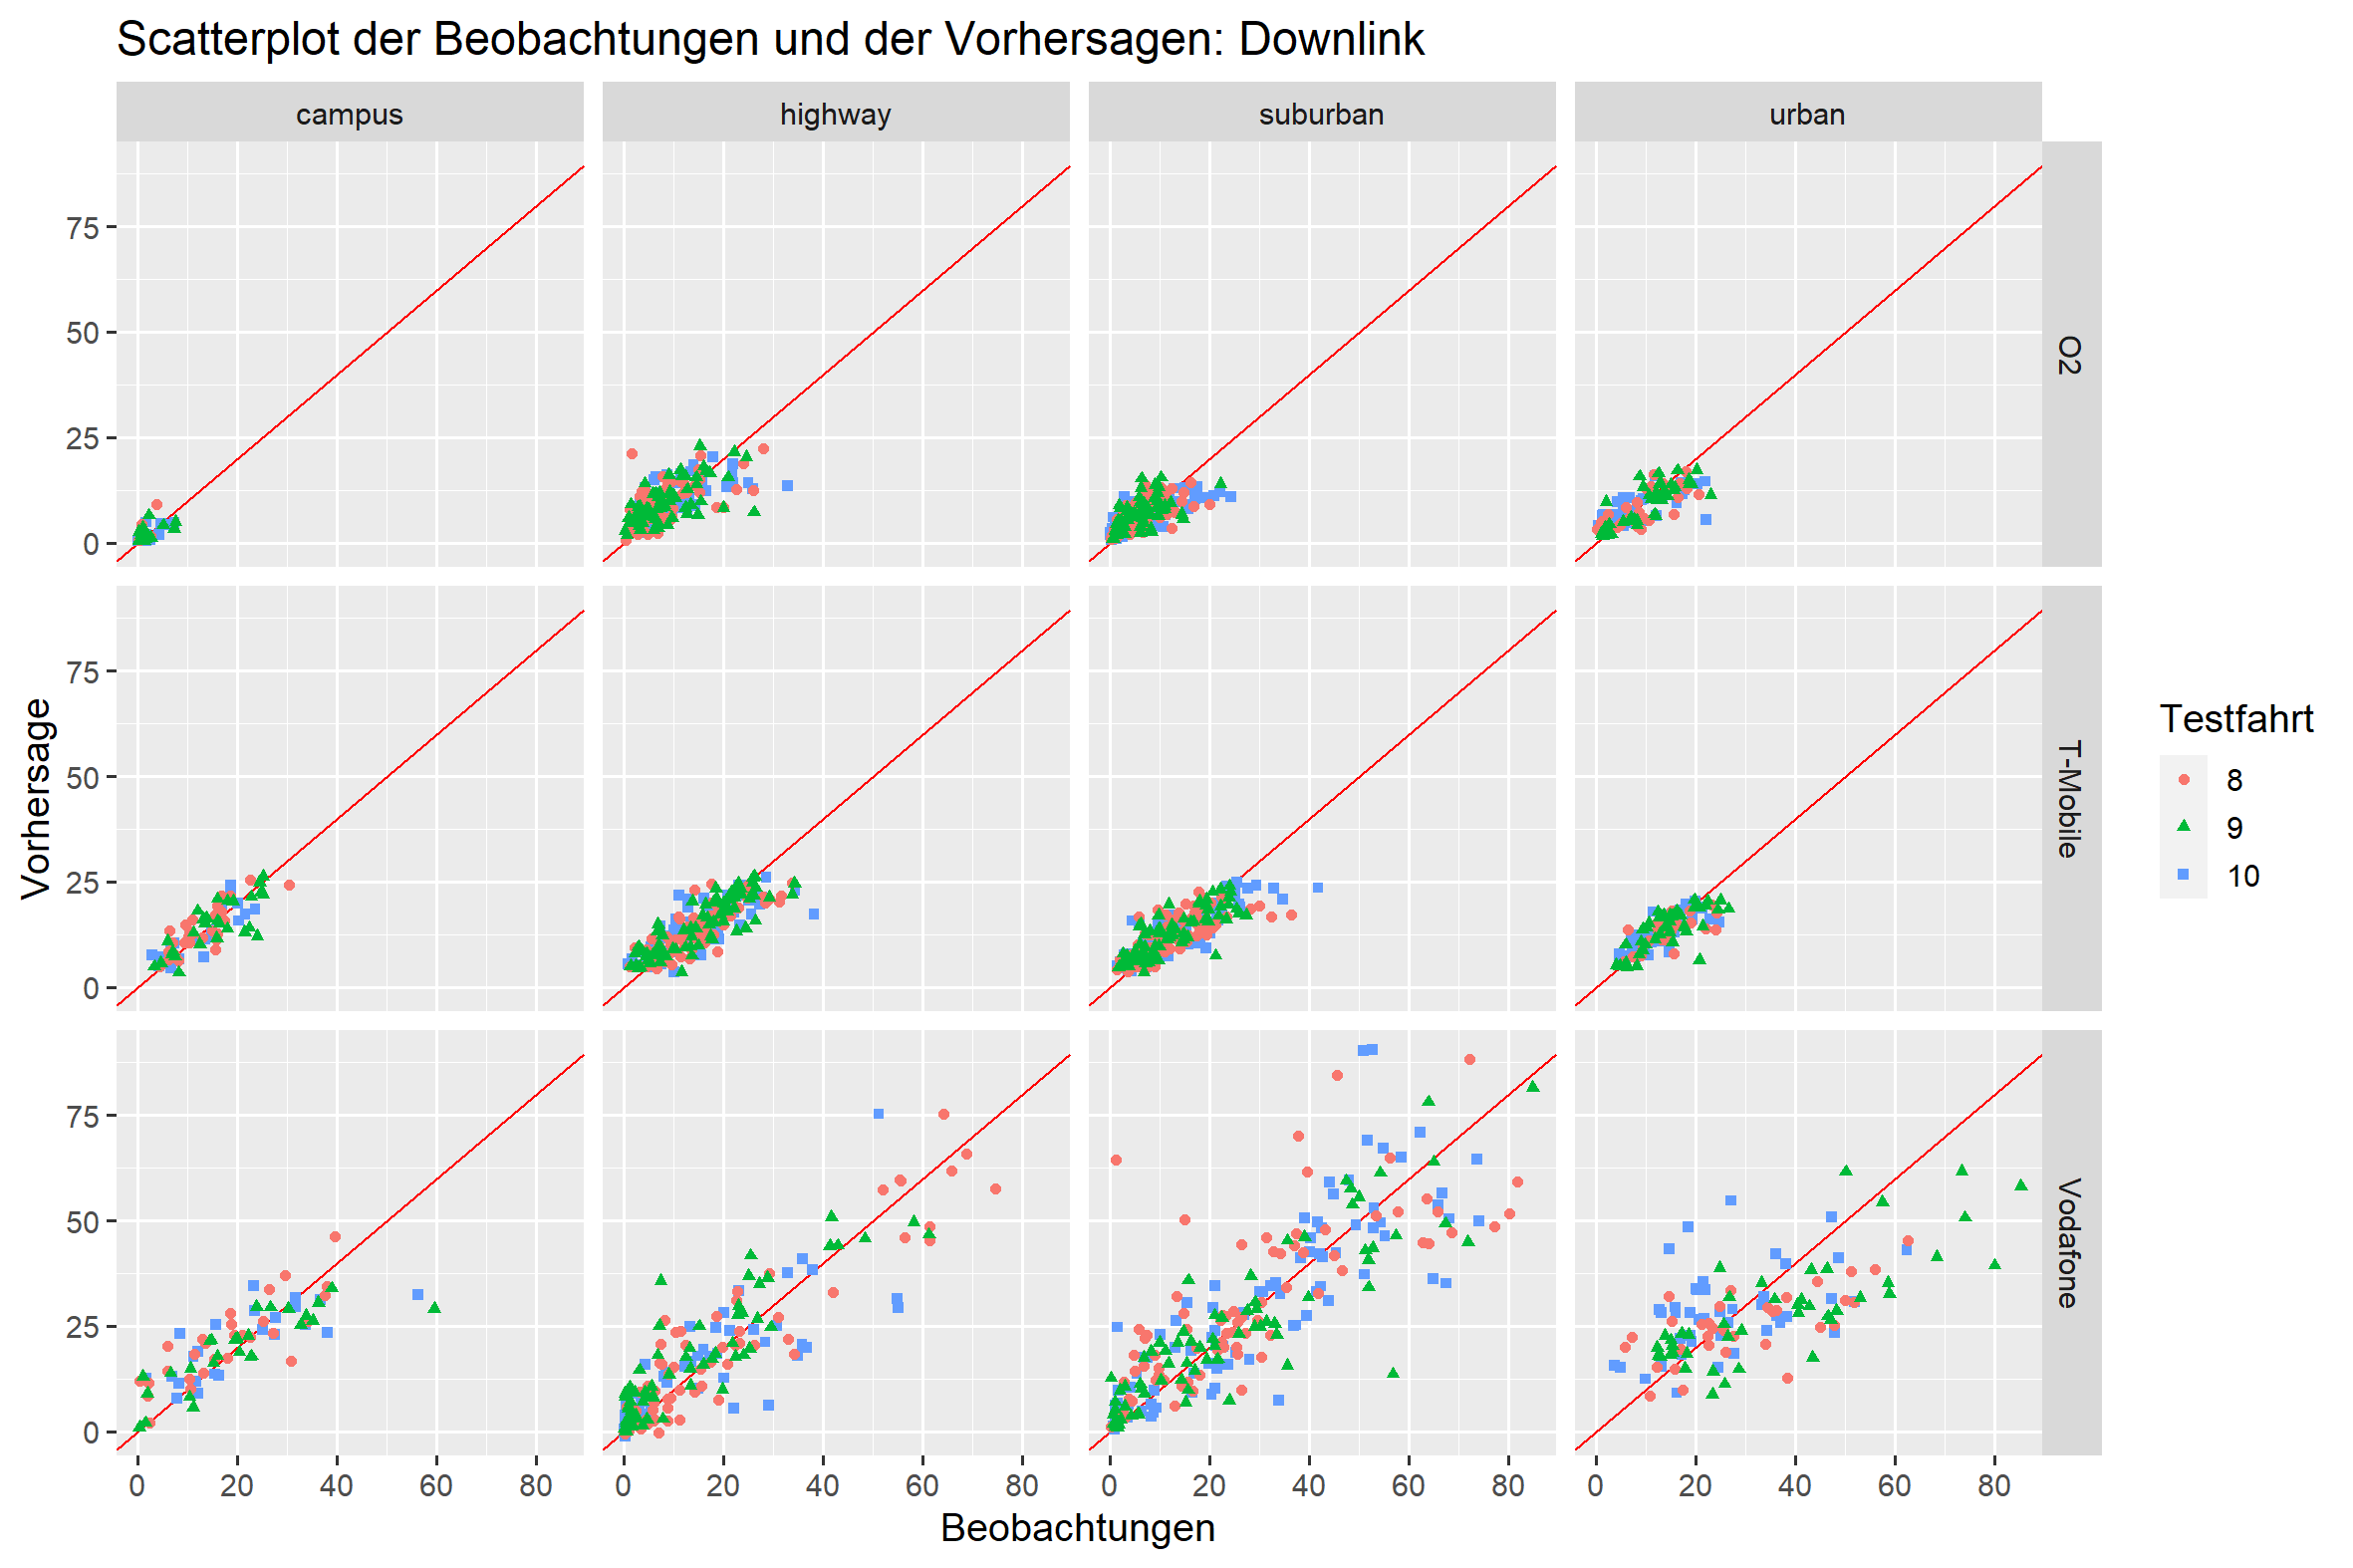
\includegraphics[width=\textwidth]{abbildungen/xgboost_predictions_dl}
\end{subfigure}
\caption{Out-of-Sample Vorhersagen der Datenraten f\"ur Extreme Gradient Boosting.}
\label{fig:datarate-predictions-xgboost}
\end{figure}

\subsubsection{Regression mit ARMA-Fehlern}

\begin{figure}
\centering
\begin{subfigure}{\textwidth}
    \centering
    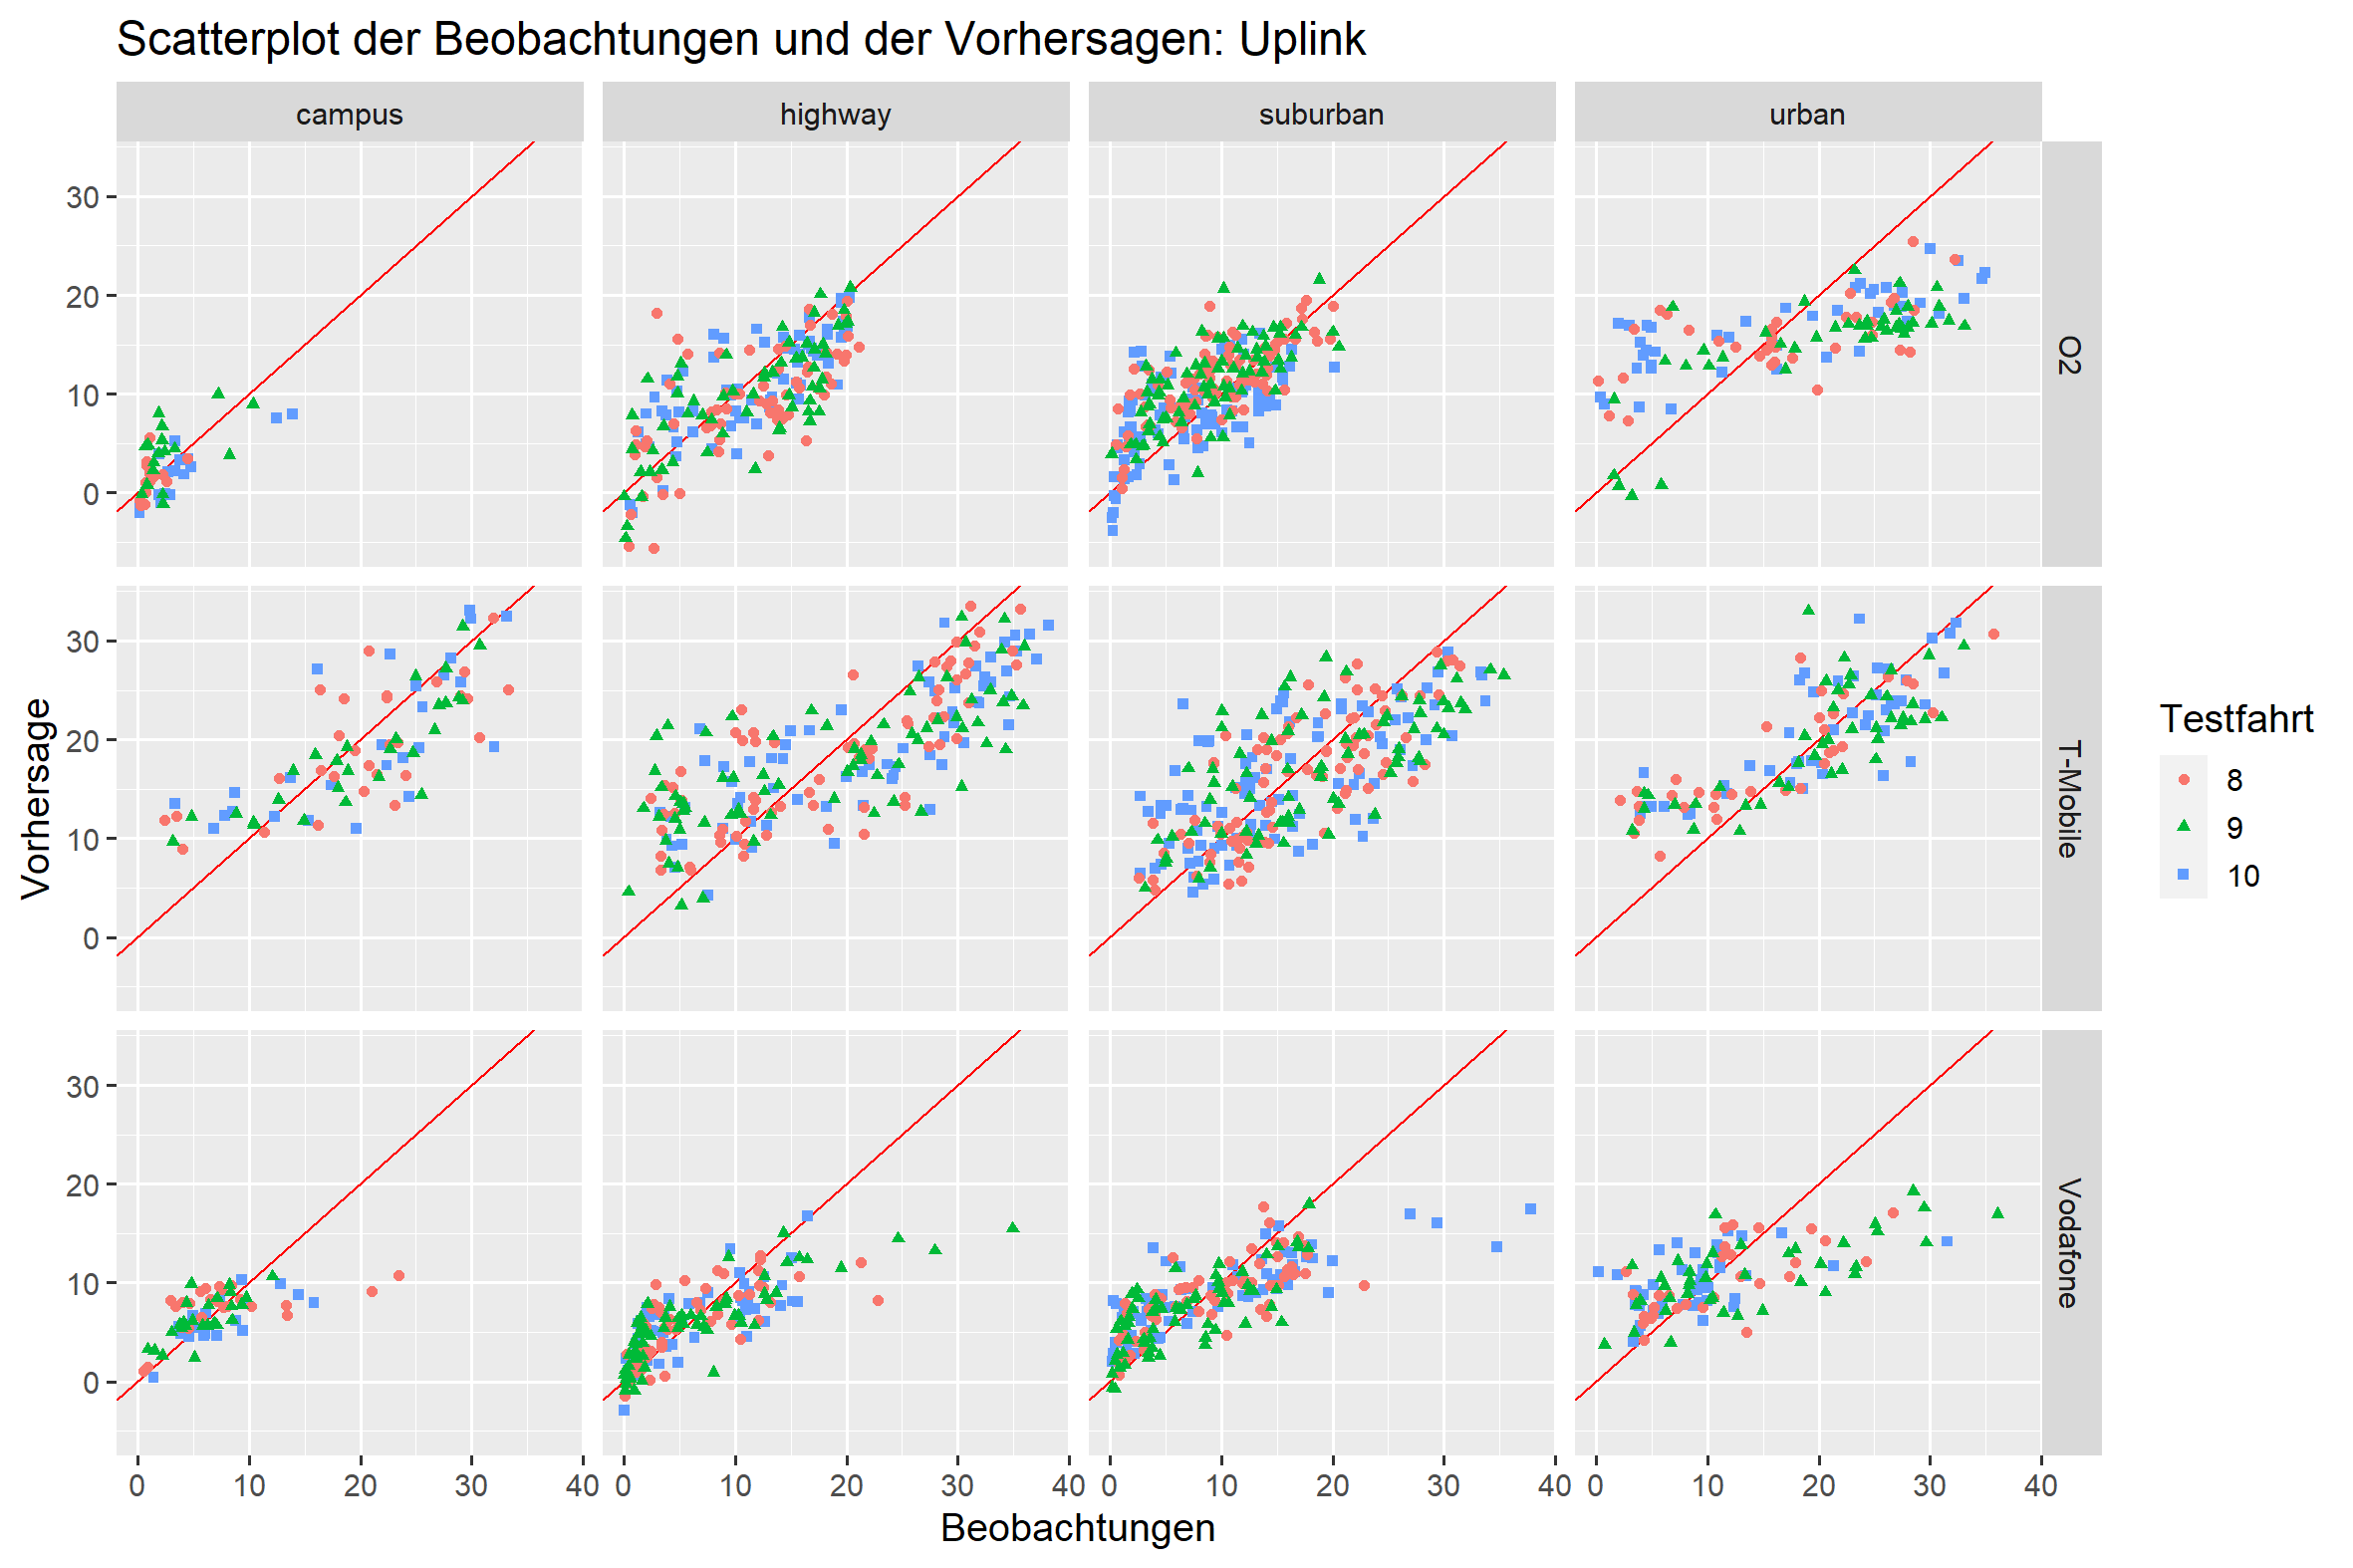
\includegraphics[width=\textwidth]{abbildungen/arma_predictions_ul}
\end{subfigure}
\begin{subfigure}{\textwidth}
    \centering
    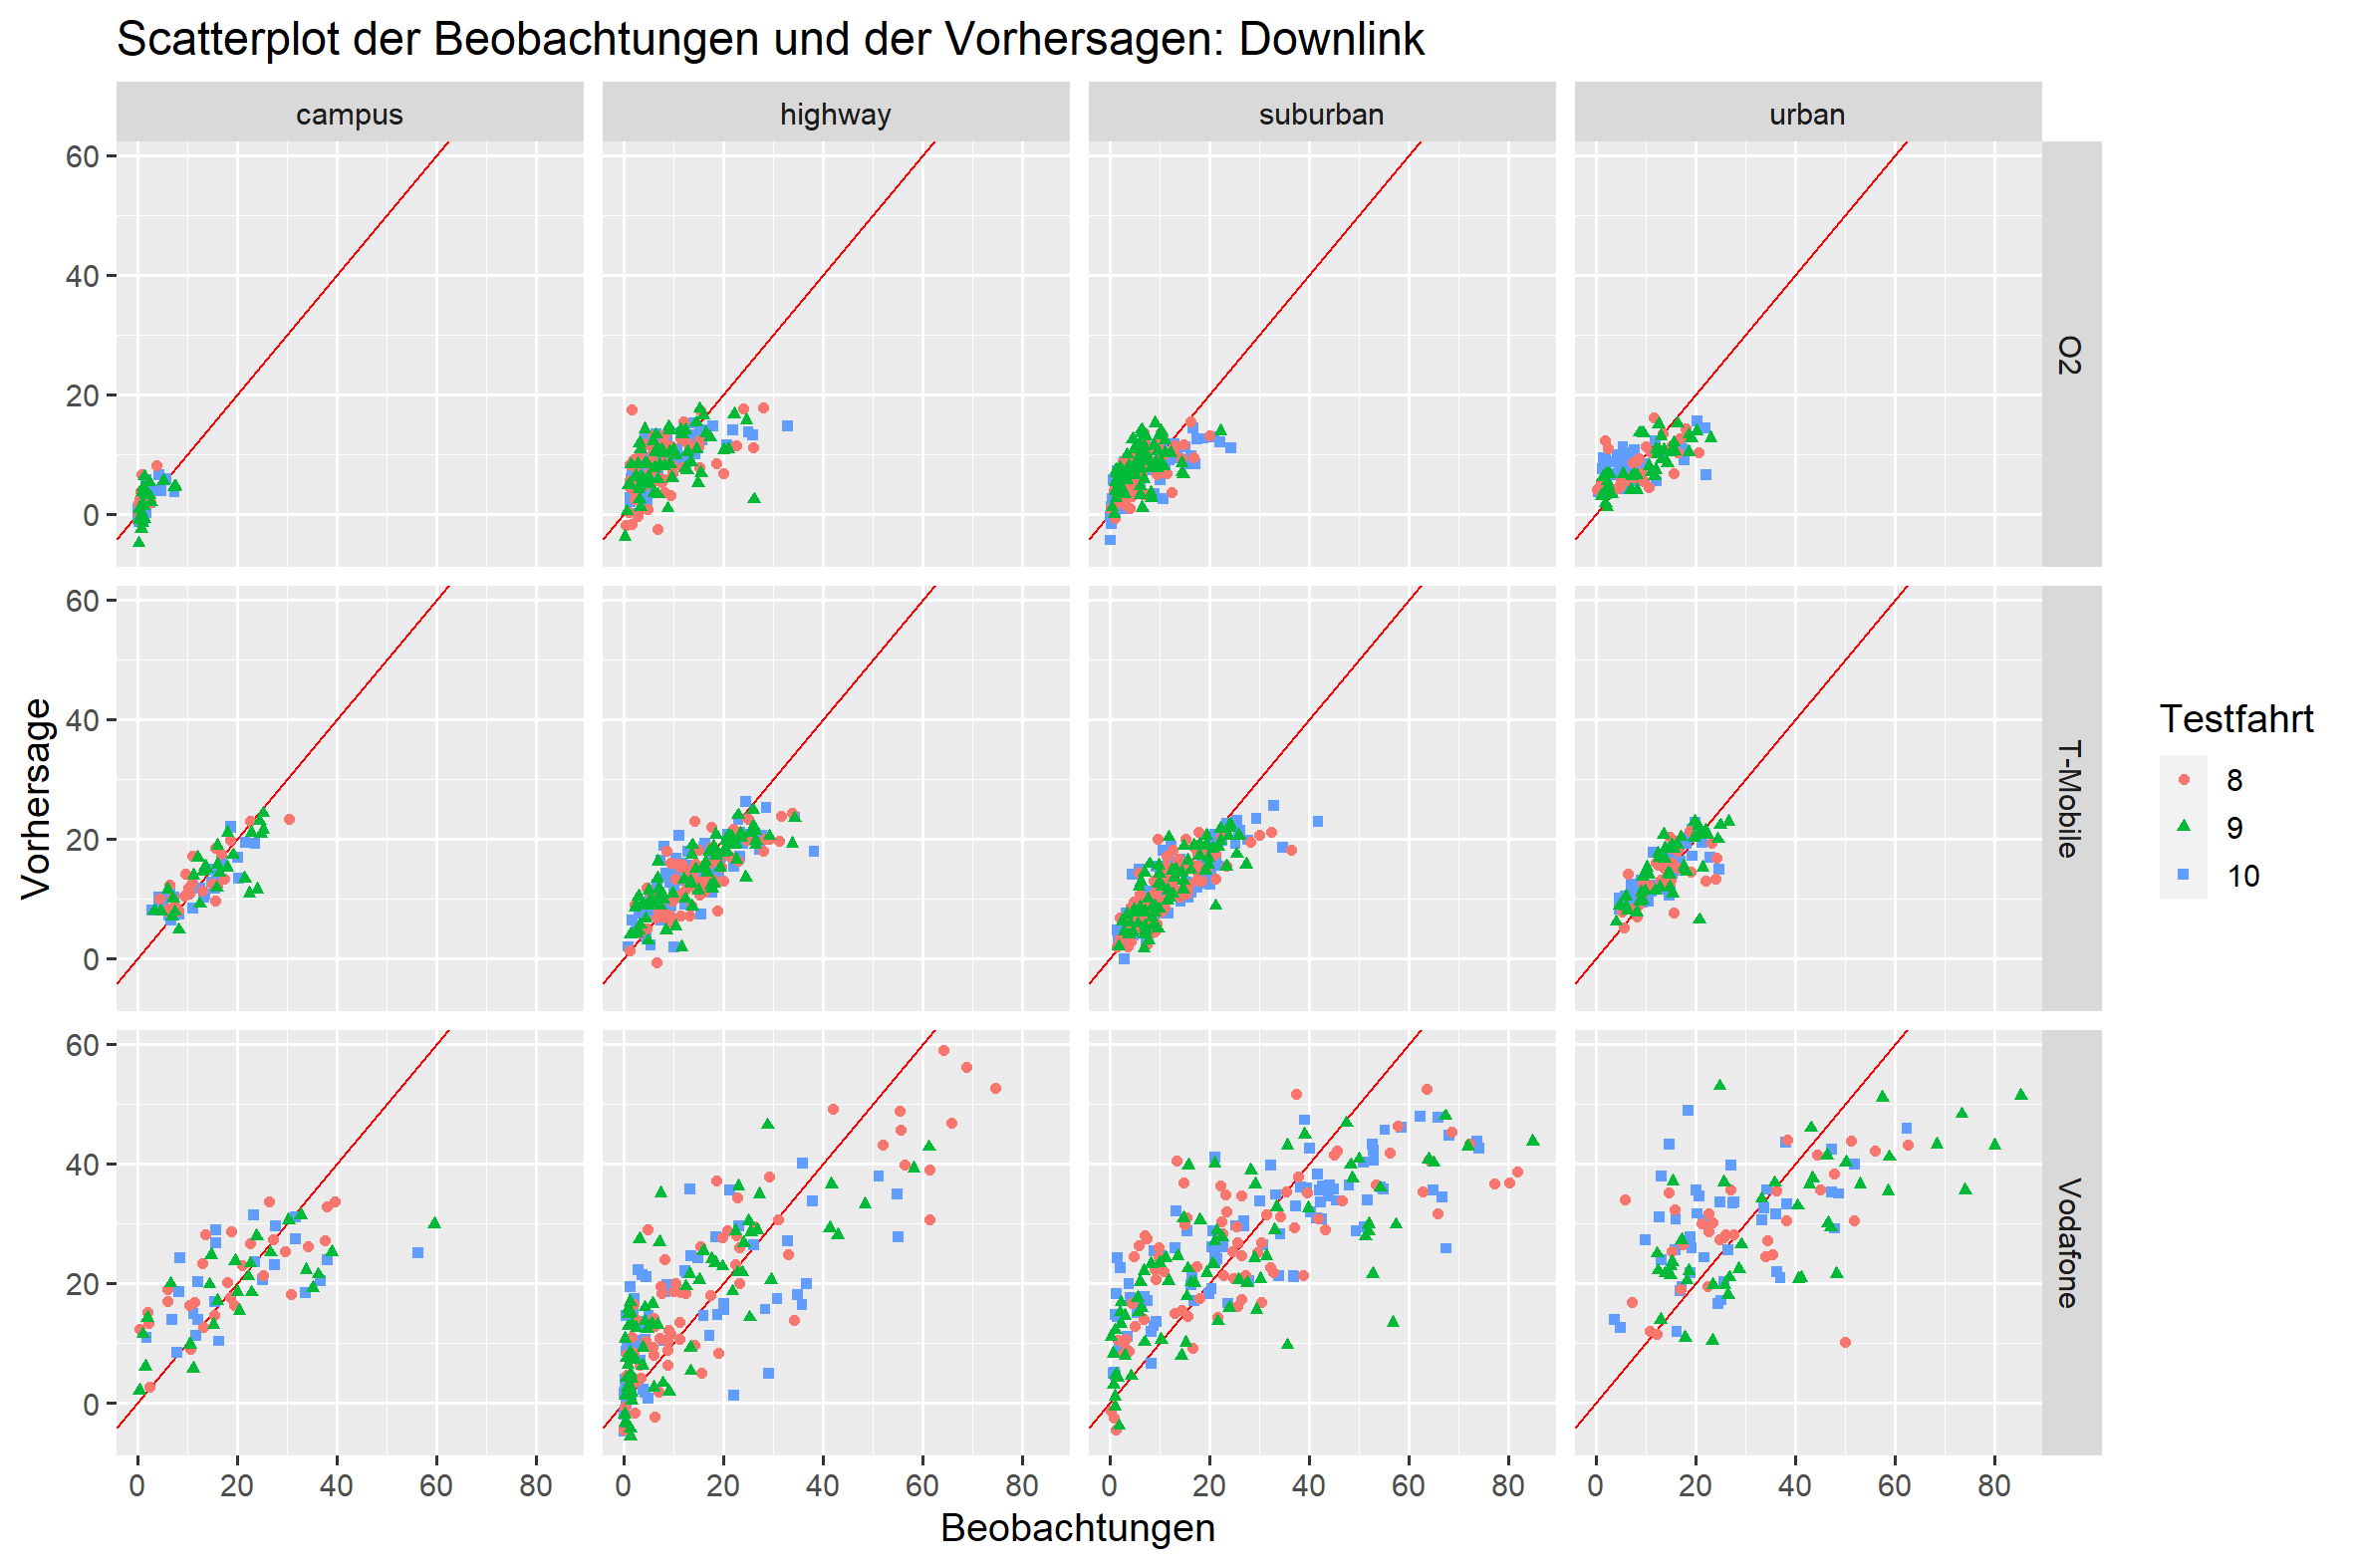
\includegraphics[width=\textwidth]{abbildungen/arma_predictions_dl}
\end{subfigure}
\caption{Out-of-Sample Vorhersagen der Datenraten f\"ur die Regression mit ARMA-Fehlern.}
\label{fig:datarate-predictions-arma}
\end{figure}

\subsubsection{Modellvergleich}

\begin{figure}
\centering
\begin{subfigure}{0.49\textwidth}
    \centering
    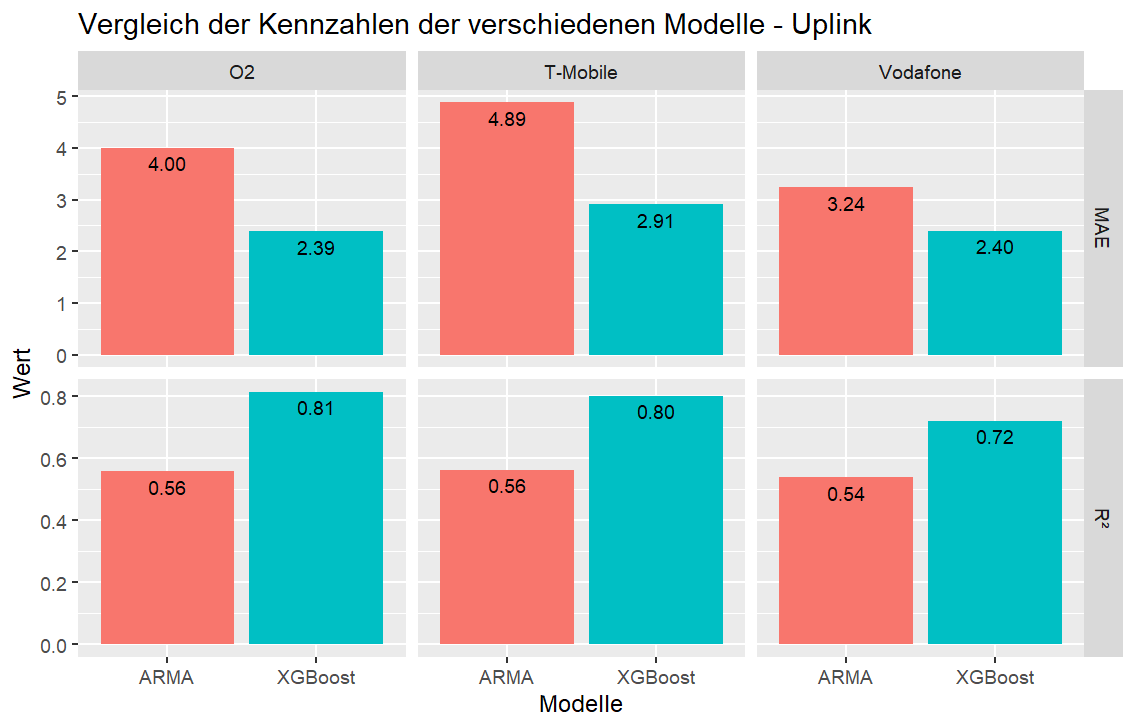
\includegraphics[width=\textwidth]{abbildungen/kennzahlen_vergleich_uplink}
\end{subfigure}
\begin{subfigure}{0.49\textwidth}
    \centering
    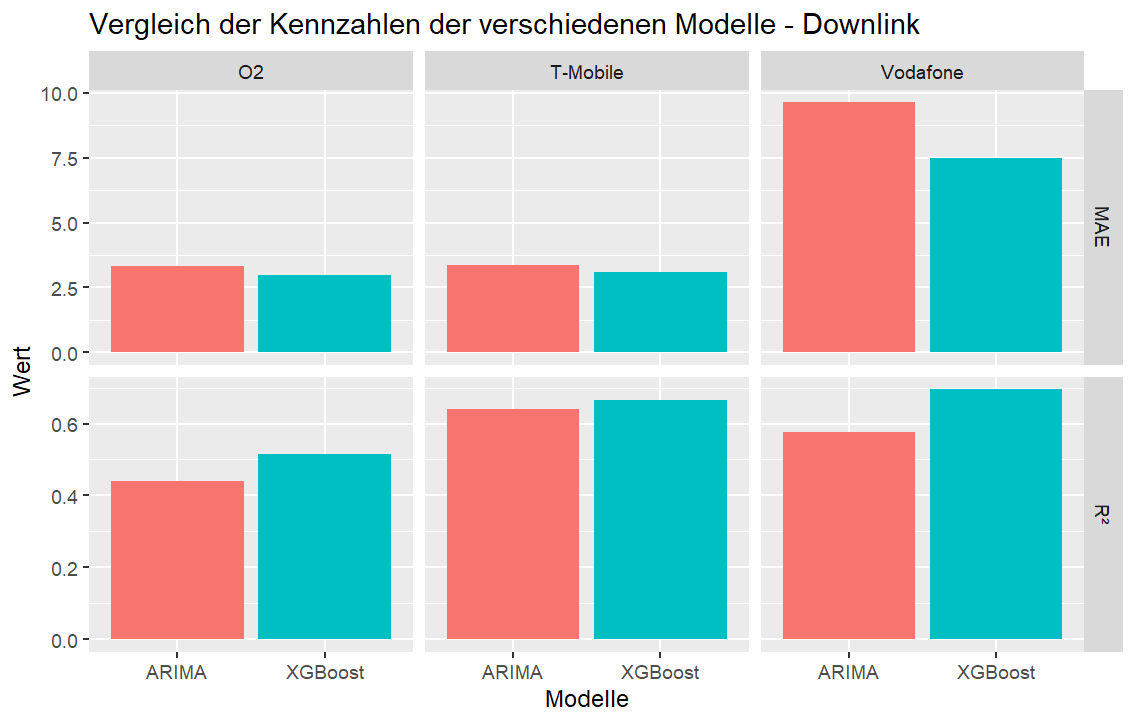
\includegraphics[width=\textwidth]{abbildungen/kennzahlen_vergleich_downlink}
\end{subfigure}
\caption{Vergleich der Kennzahlen f\"ur die Pr\"adiktion der Upload- und Download-Raten.}
\label{fig:kennzahlen-datarate}
\end{figure}

\begin{figure}
\centering
\begin{subfigure}{\textwidth}
    \centering
    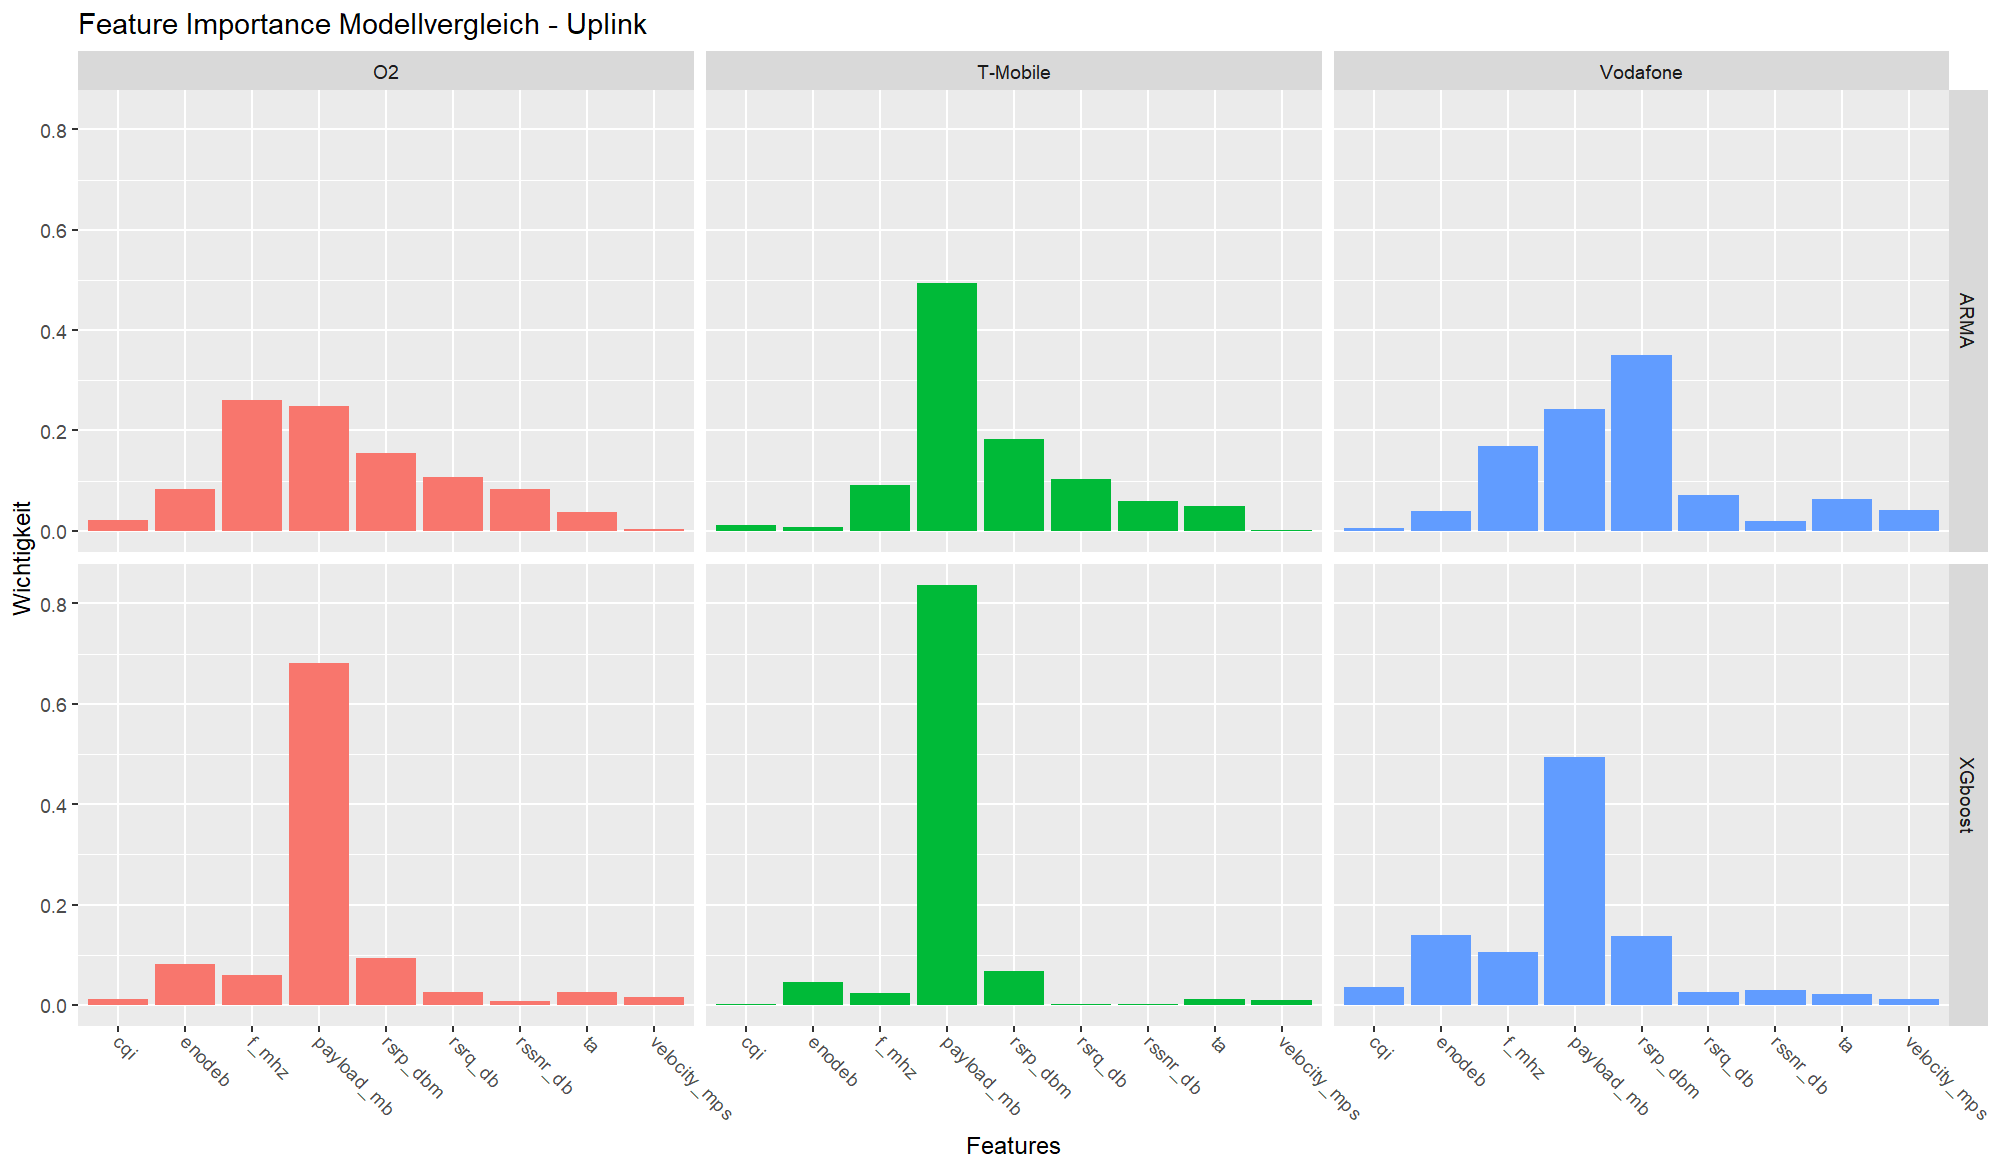
\includegraphics[width=\textwidth]{abbildungen/feature_importance_modellvergleich_uplink}
\end{subfigure}
\begin{subfigure}{\textwidth}
    \centering
    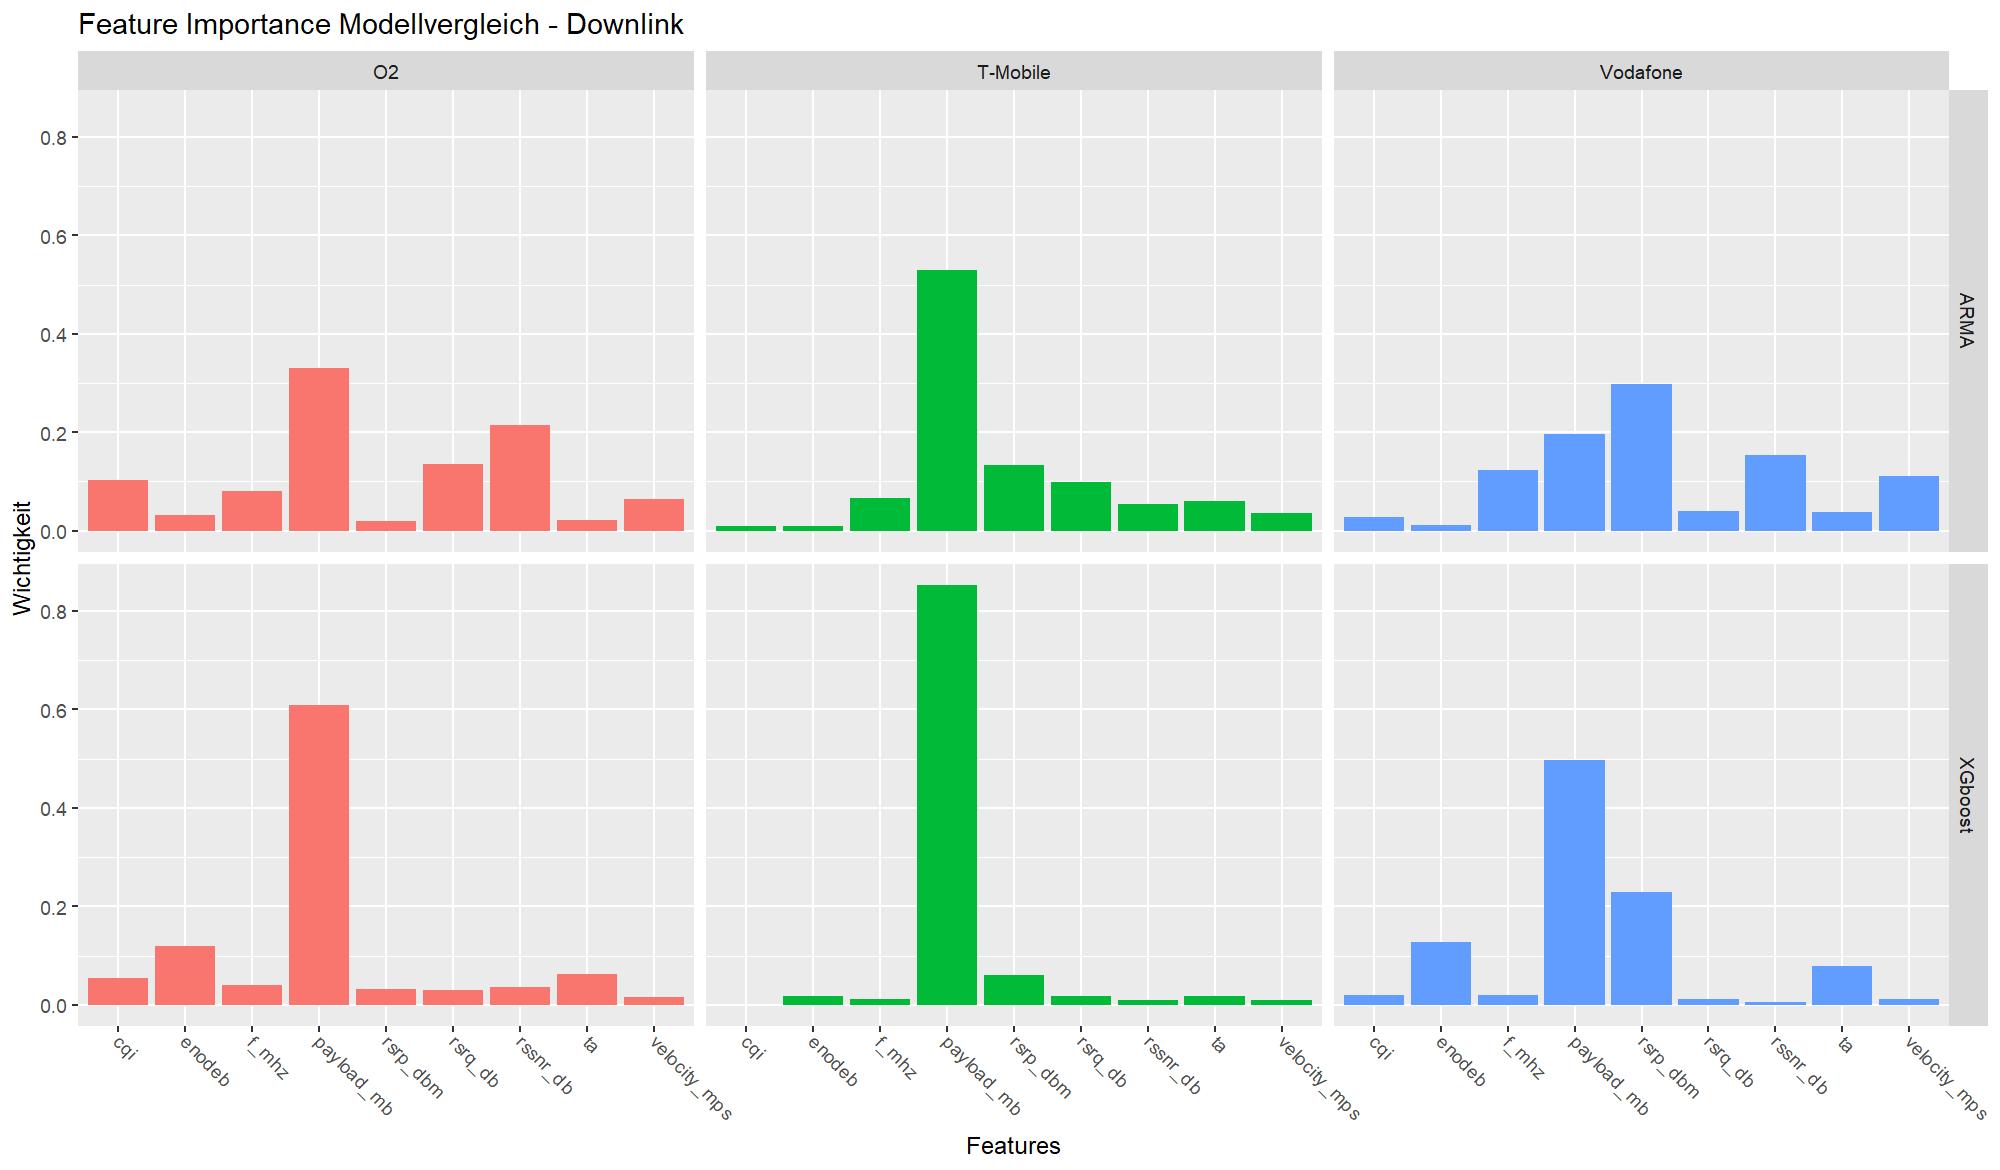
\includegraphics[width=\textwidth]{abbildungen/feature_importance_modellvergleich_downlink}
\end{subfigure}
\caption{Feature Importance der Modelle zur Datenratenpr\"adiktion.}
\label{fig:feature-importance-datenraten}
\end{figure}

\subsection{Vorhersage der eNodeB-Verbindungsdauern}

\begin{figure}
    \centering
    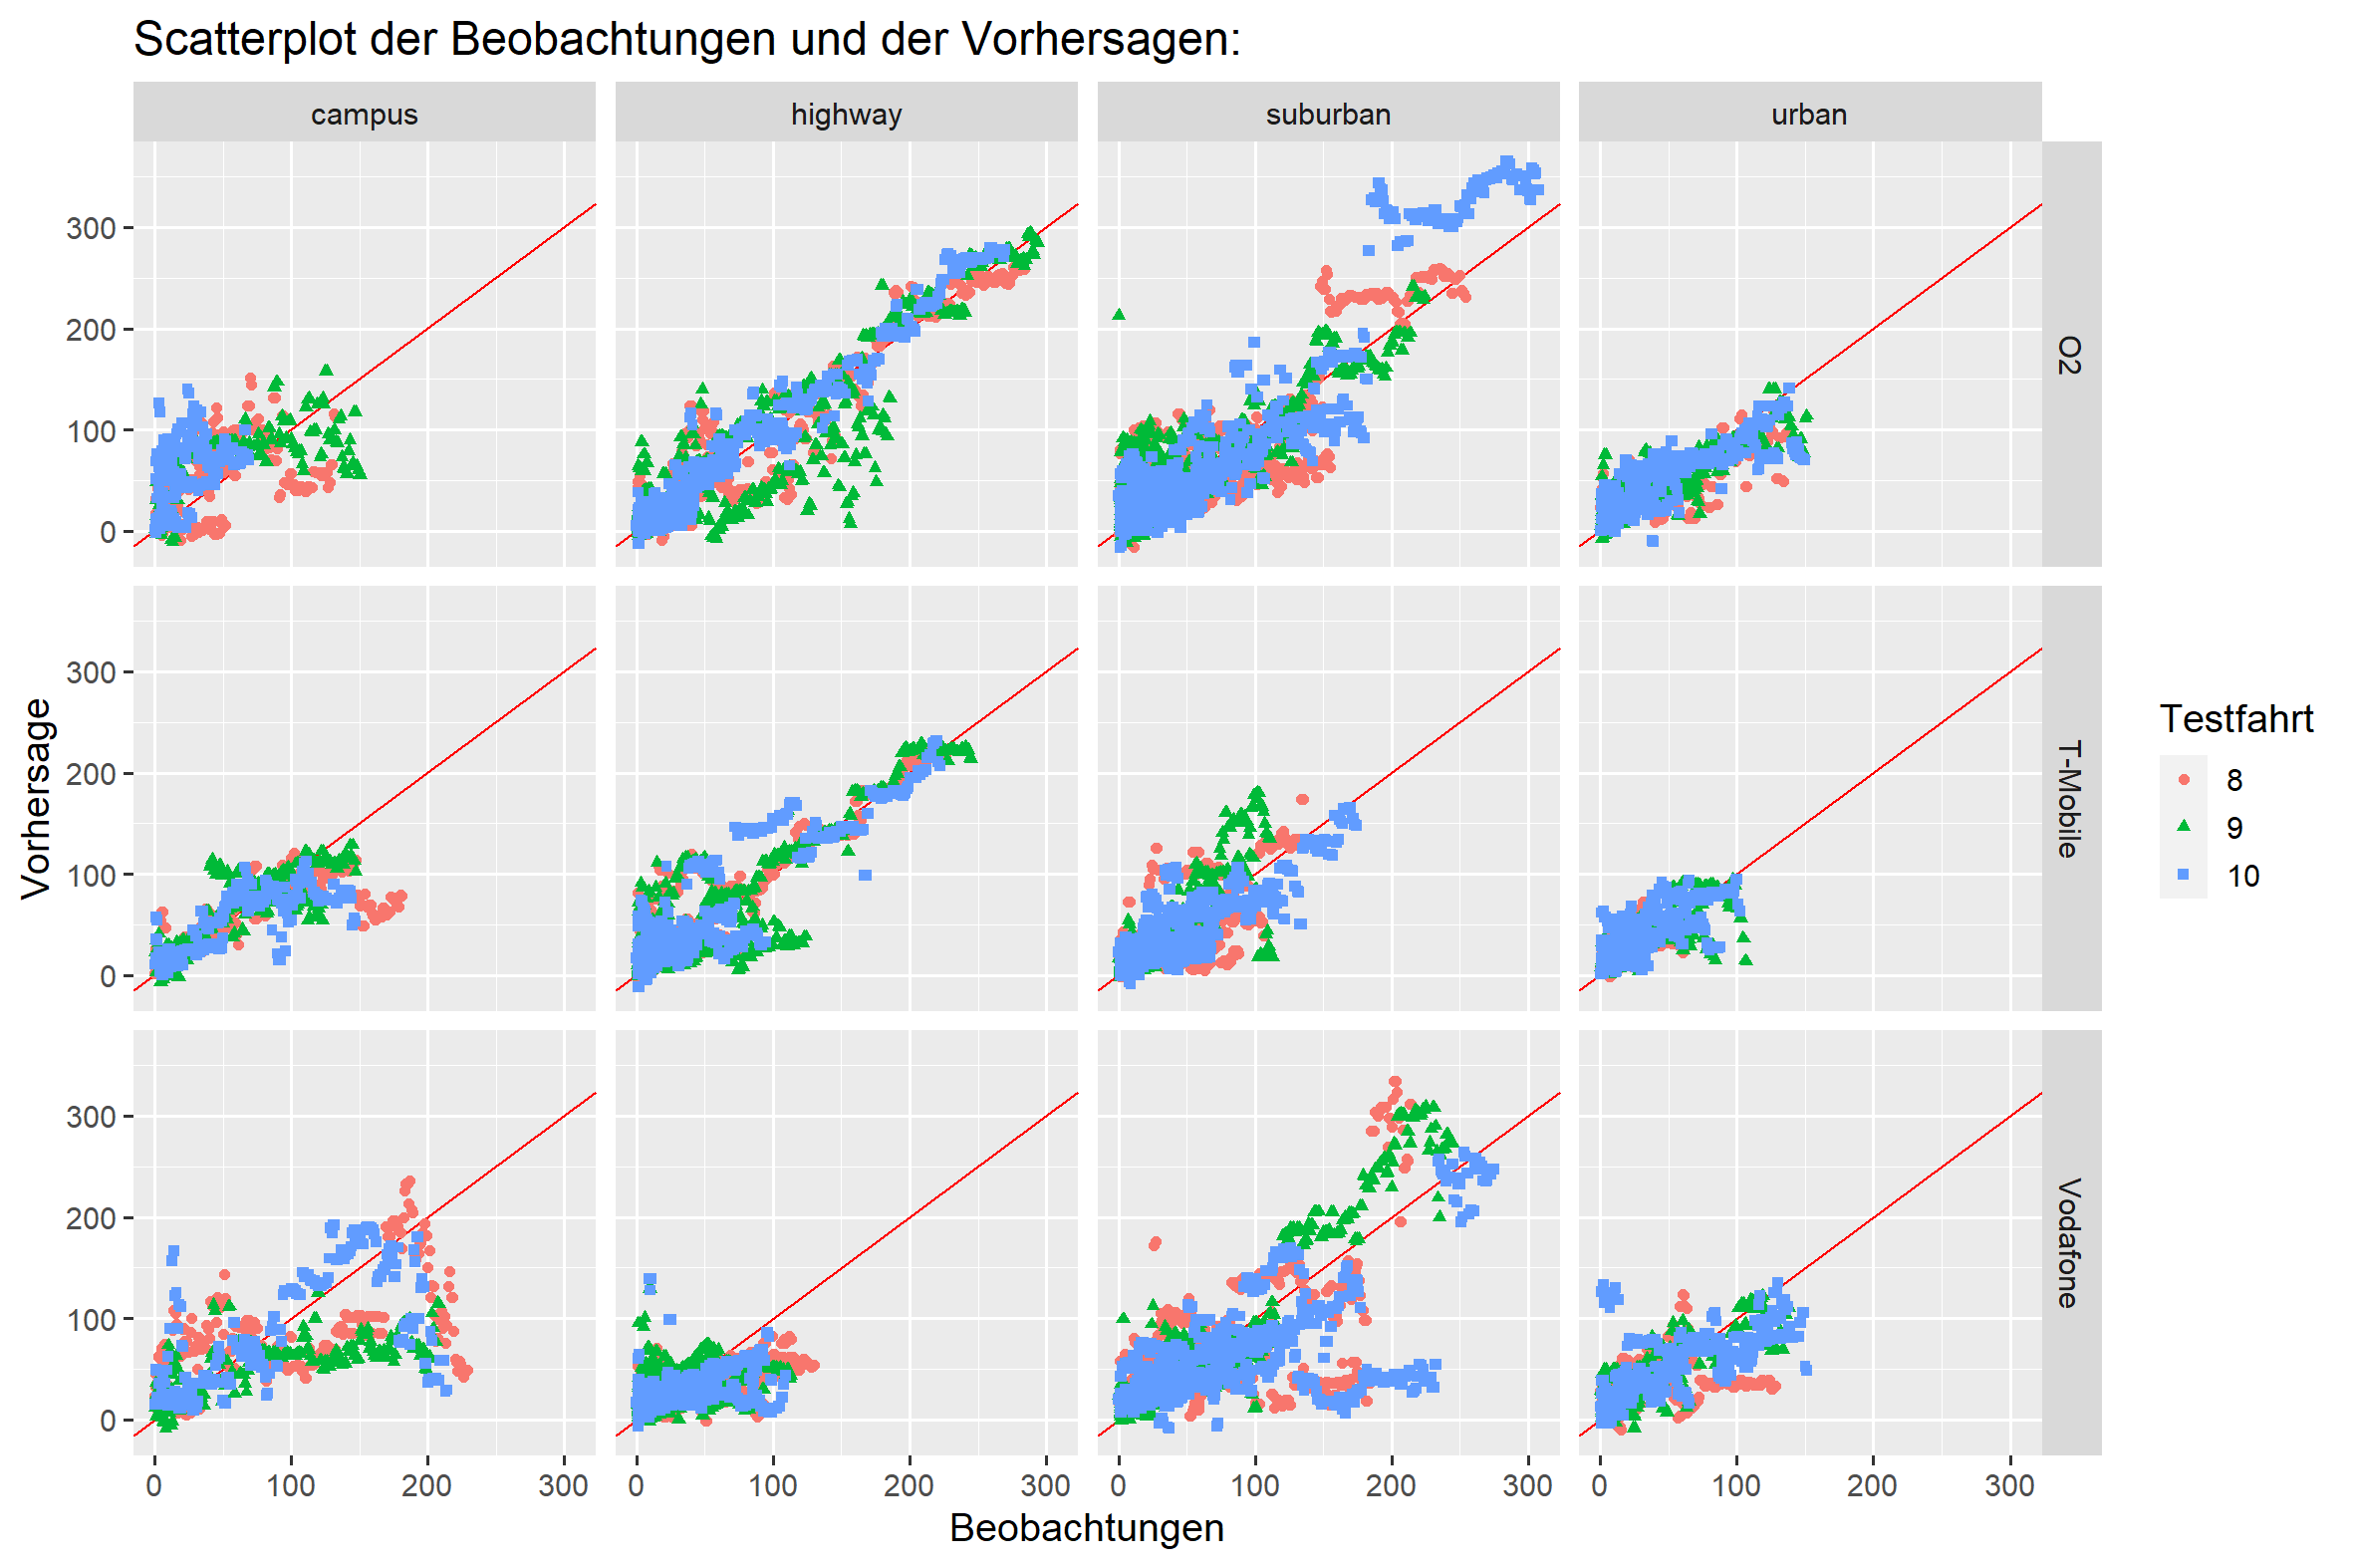
\includegraphics[width=\textwidth]{abbildungen/predictions_linklifetime}
    \caption{Out-of-Sample Vorhersagen der eNodeB-Verbindungsdauern.}
    \label{fig:link-lifetime-predictions}
\end{figure}